\chapter{Performance Analysis}
\label{cha:pa}

In this chapter, we will examine \textit{project name}'s performance. Firstly,
we present the difference in execution time between a secured binary and a non-secure
one giving great importance to the time overhead. Secondly, we present the
difference in size between the produced binaries. Lastly, we will see an
analysis of the obtained results as well as some optimization ideas to further
improve the performance of the project.

To perform a correct and realistic analysis of the performance of the project
$13$ algorithms plus $4$ variations with indirect jumps are provided. Each algorithm
has been compiled and run both in secure and non-secure mode. All tests have
been conducted on the aforementioned Espressif's board.

\section{Time Performances}
\label{sec:pa_time}

In this section, we will see how \textit{project name}'s infrastructure affects the
execution time of the code. (two histograms depicting test results can be seen in
Figures \ref{fig:lowtime} and \ref{fig:hightime}).

\begin{figure}[htbp]
  \centering
  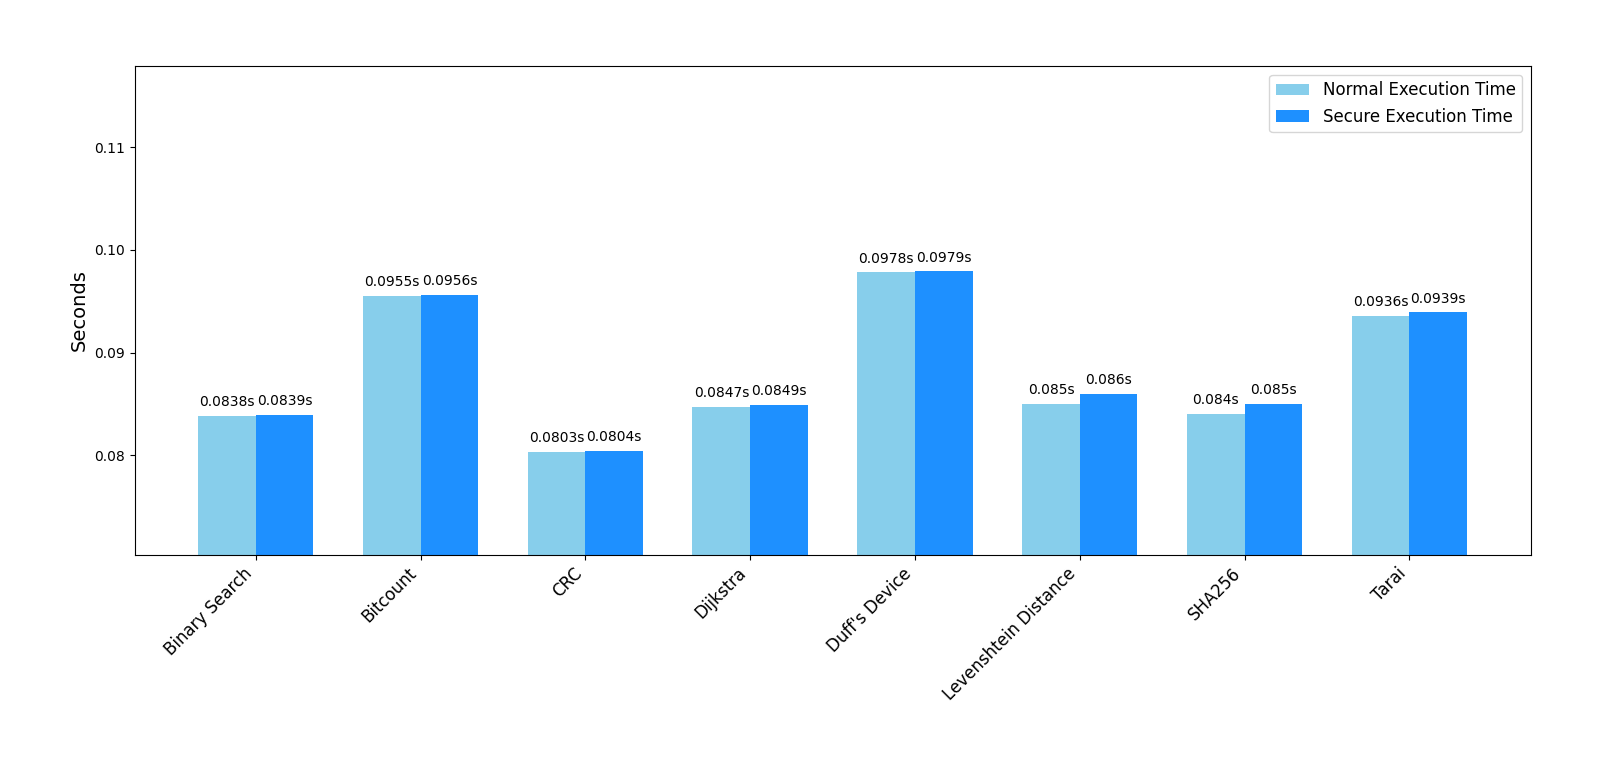
\includegraphics[width=.9\linewidth]{images/low_execution.png}
  \caption{Comparison between binaries execution times (low times)}
  \label{fig:lowtime}
\end{figure}

\begin{figure}[htbp]
  \centering
  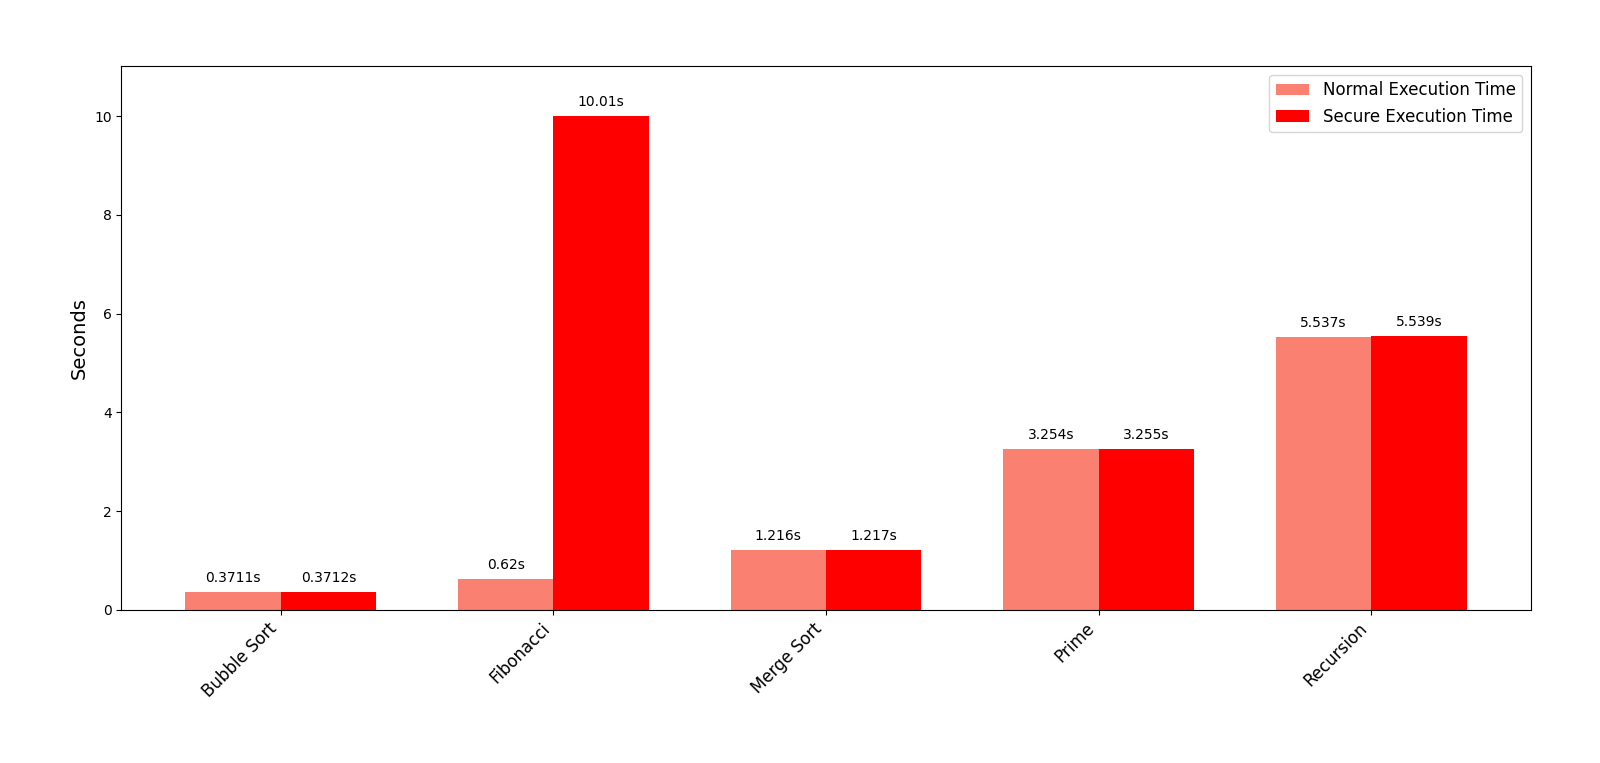
\includegraphics[width=.9\linewidth]{images/high_execution.png}
  \caption{Comparison between binaries execution times (medium and high times)}
  \label{fig:hightime}
\end{figure}

As we can see in Table \ref{tab:times}, in most cases the time overhead affects the
fourth or fifth digit resulting in an unnoticeable increase in execution time.
However, in two cases the time overhead is very large and slows the execution by
a relevant factor.

It is straightforward to understand why the overhead is smaller for algorithms like
\textit{Binary Search} and \textit{Duff's Device} since these programs perform few
jumps and most of the computation is performed inside a while or for loop so,
the overhead given by the instrumentation is unnoticeable if compared to the
total execution time.

Instead, examples like \textit{Prime} and \textit{Recursive} are a bit trickier.
Since these algorithms work with a recursive approach we expect them to perform
many control transfer instructions Consequently, we expect the time required for
the context switch and the edge controls to be somewhat impactful. However, results
show that even in these cases the difference is barely noticeable\footnote{In
these cases instead of impacting the fourth/fifth digit the overhead impacts the
second or third digit.}. The reason could be due to the processor's frequency which,
in the case of \textit{Espressif's ESP32-C3}, is $160 \ MHz$. This means that even
the CPU is able to perform to execute the secure and non-secure binaries in a similar
time. For example, the \textit{Recursion} algorithm performs $\sim 4000$ jump
instructions and $\sim 4000$ return instructions which translates to $\sim 8000$
edge controls and $\sim 16000$ context switches. However, if we compare those
numbers to the $160$ million operations the processor can perform in a second we
see why the time overhead is so small. In fact, if we compute
$\frac{8000}{160000000}$ we discover that the utilized processor is able to
perform $8000$ instructions in $0.00005$ seconds.

Two peculiar cases are the ones of the \textit{Fibonacci} and \textit{Fibonacci
Indirect} algorithms, in these cases, we can see that the overheads are
$1523.24\%$ and $77.97\%$ respectively. The possible reason for these enormous overheads
is that these algorithms make two recursive calls each time so we end up with a staggering
amount of jump and return instructions. This leads to many edge controls and the
execution is strongly affected by this.

Overall, \textit{project name} achieved an average time overhead of $94.38\%$
with a standard deviation of $368.68$. However, if we do not take into account
the outliers we can see that the median is $0.036\%$. These results clearly show
that \textit{project name}'s time overhead is almost unnoticeable in many cases
but, this also demonstrates that the project strongly suffers from deeply recursive
algorithms.

\begin{table}
  \centering
  \begin{tabular}{|c|c|c|c|}
    \hline
    \textbf{Algorithm}          & \textbf{Normal run time (s)} & \textbf{Secure run time (s)} & \textbf{Time Overhead} \\
    \hhline{====} Binary Search & 0.08387                      & 0.08388                      & $0.012\%$              \\
    \hline
    Bitcount                    & 0.0955                       & 0.0956                       & $0.11\%$               \\
    \hline
    Bubble Sort                 & 0.37113                      & 0.37116                      & $0.008\%$              \\
    \hline
    CRC                         & 0.08025                      & 0.08026                      & $0.012\%$              \\
    \hline
    Dijkstra                    & 0.0847                       & 0.0849                       & $0.236\%$              \\
    \hline
    Duff's Device               & 0.097795                     & 0.097799                     & $0.0041\%$             \\
    \hline
    Fibonacci                   & 0.6166                       & 10.0089                      & $1523.24\%$            \\
    \hline
    Fibonacci Indirect          & 0.0849                       & 0.1511                       & $77.97\%$              \\
    \hline
    Levenshtein Distance        & 0.085                        & 0.086                        & $1.176\%$              \\
    \hline
    Merge Sort                  & 1.216                        & 1.217                        & $0.0822\%$             \\
    \hline
    Merge Sort Indirect         & 1.2168                       & 1.2169                       & $0.0082\%$             \\
    \hline
    Prime                       & 3.254                        & 3.255                        & $0.03\%$               \\
    \hline
    Prime Indirect              & 3.253                        & 3.254                        & $0.03\%$               \\
    \hline
    Recursion                   & 5.537                        & 5.539                        & $0.036\%$              \\
    \hline
    Recursion Indirect          & 5.537                        & 5.539                        & $0.036\%$              \\
    \hline
    SHA256                      & 0.084                        & 0.085                        & $1.19\%$               \\
    \hline
    Tarai                       & 0.0936                       & 0.0939                       & $0.32\%$               \\
    \hline
  \end{tabular}
  \caption{Test results for execution time}
  \label{tab:times}
\end{table}

Lastly, in Table \ref{tab:othertimes} we can see the time required to instrument
the code, extract the CFG, and perform the simulation. As we can see the
instrumentation and CFG extraction phases always require less than a fraction of
a second to finish. However, we must take into consideration that the tested
algorithms are composed of few lines of code and the situation could change if
we were to instrument a firmware composed of thousands of lines. The simulation instead
requires a lot of time, even algorithms that run in a second or less require a
few seconds to simulate. This is due to the logging required to extract the indirect
jump destinations that affect the time performances seriously. However, we can accept
this result since the simulation is run only once and the logging is removed from
the final binary so that this overhead is not affecting the actual execution.

\begin{table}
  \centering
  \begin{tabular}{|c|c|c|c|}
    \hline
    \textbf{Algorithm}          & \textbf{Instrumentation (s)} & \textbf{Simulation (s)} & \textbf{CFG extraction (s)} \\
    \hhline{====} Binary Search & 0.00296                      & no ind jumps            & 0.00174                     \\
    \hline
    Bitcount                    & 0.00196                      & no ind jumps            & 0.00153                     \\
    \hline
    Bubble Sort                 & 0.00302                      & no ind jumps            & 0.00175                     \\
    \hline
    CRC                         & 0.00203                      & no ind jumps            & 0.00154                     \\
    \hline
    Dijkstra                    & 0.00264                      & no ind jumps            & 0.00182                     \\
    \hline
    Duff's Device               & 0.00265                      & no ind jumps            & 0.00163                     \\
    \hline
    Fibonacci                   & 0.00209                      & no ind jumps            & 0.00149                     \\
    \hline
    Fibonacci Indirect          & 0.00202                      & 130.5567                & 0.07037                     \\
    \hline
    Levenshtein Distance        & 0.00255                      & no ind jumps            & 0.00167                     \\
    \hline
    Merge Sort                  & 0.00354                      & no ind jumps            & 0.00178                     \\
    \hline
    Merge Sort Indirect         & 0.0036                       & 4.6394                  & 0.00273                     \\
    \hline
    Prime                       & 0.00214                      & no ind jumps            & 0.00168                     \\
    \hline
    Prime Indirect              & 0.00208                      & 11.4051                 & 0.00451                     \\
    \hline
    Recursion                   & 0.00202                      & no ind jumps            & 0.00159                     \\
    \hline
    Recursion Indirect          & 0.00202                      & 23.2751                 & 0.00875                     \\
    \hline
    SHA256                      & 0.00411                      & no ind jumps            & 0.00189                     \\
    \hline
    Tarai                       & 0.00198                      & no ind jumps            & 0.00152                     \\
    \hline
  \end{tabular}
  \caption{Test result for instrumentation phases times}
  \label{tab:othertimes}
\end{table}

\section{Memory Overhead}
\label{sec:pa_memory}

In this section, we will see how \textit{project name} affects the size of the produced
binary (a histogram depicting test results can be seen in Figure
\ref{fig:binsize}).

\begin{figure}[htbp]
  \centering
  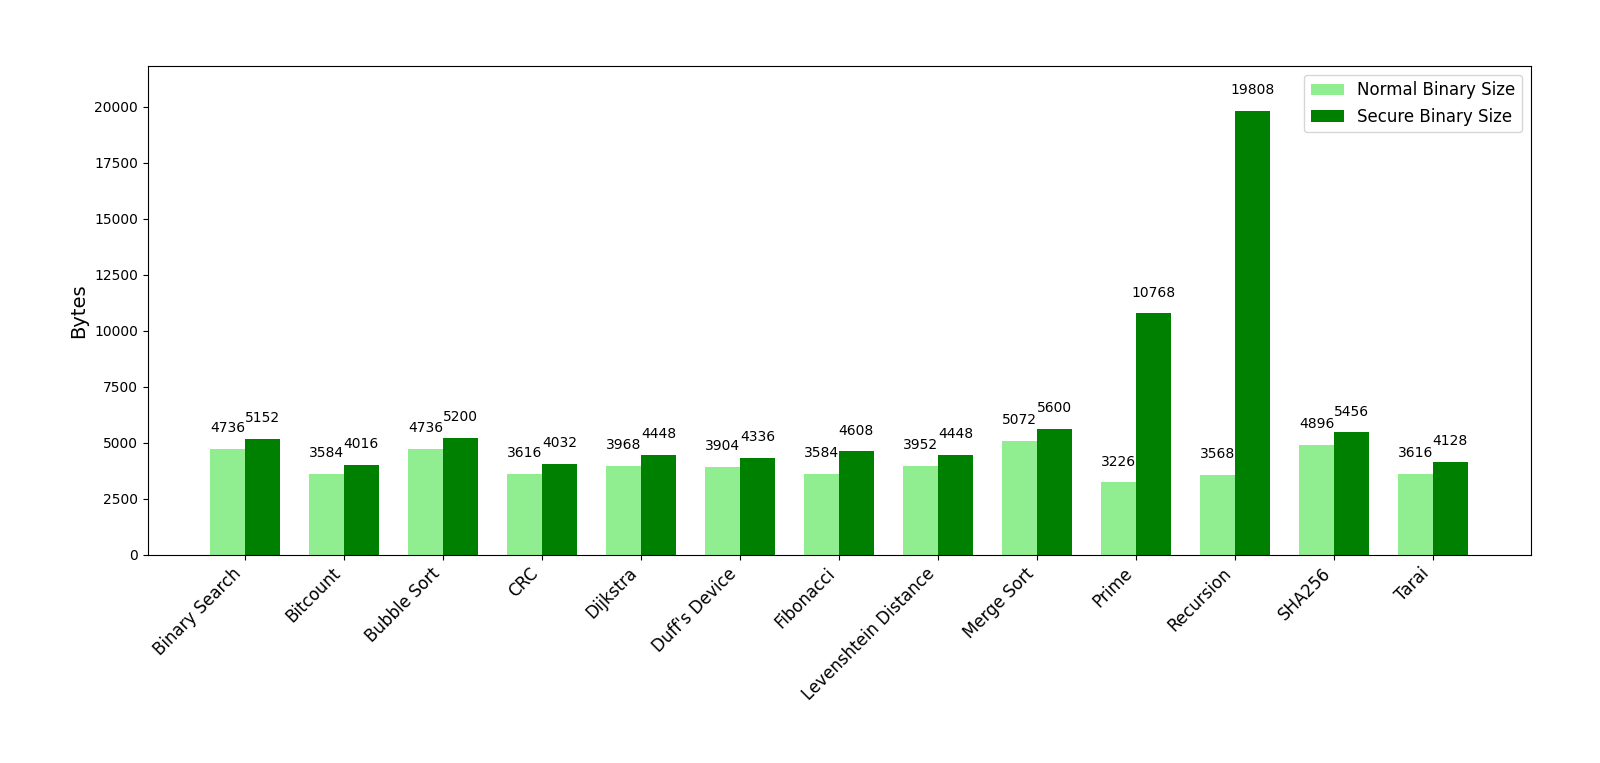
\includegraphics[width=.9\linewidth]{images/bin_sizes.png}
  \caption{Comparison between binaries size}
  \label{fig:binsize}
\end{figure}

As we can see in Table \ref{tab:binsize}, in most cases the size of the binary increases
by $\sim 10\%$. This is due to the Shadow Stack, CFG, and the instructions added
during instrumentation.

As for the time analysis, there are some exceptions. \textit{Prime}, \textit{Recursion}
and their indirect variations present an overhead of $200\%$ or more. This
happens because these recursive algorithms perform all the jump instructions
consecutively and then all the return instructions. This means that we must allocate
a Shadow Stack big enough to store all the return addresses to ensure proper edge
controls. For example, we have seen that the \textit{Recursive} algorithm
performs $\sim 4000$ jump instructions, this means that we must create a Shadow Stack
that can store at least $4000$ addresses. Given that an address is stored as an
\textit{unsigned int}, we can easily see that a Shadow Stack that can store
$4000$ addresses occupies $4000*4 = 16000 \ \textit{Bytes}$\footnote{We multiply
by $4$ because it is the size of an \textit{unsigned int}.}. Now, if we take the
size of the secure binary for the \textit{Recursive} algorithm we can calculate
$19808 - 16000 = 380 8 \ \textit{Bytes}$, so we can see that apart from the Shadow
Stack the binary has an overhead similar to the other ones.

Note that this problem is related strictly to recursive algorithms as they perform
a high number of jumps and then they start performing the first return instruction.
However, we could have a similar problem with the Control Flow Graph as for a big
binary like a firmware we can have many different jump instructions and, as a
consequence, the CFG would increase in size.

\begin{table}
  \centering
  \begin{tabular}{|c|c|c|c|}
    \hline
    \textbf{Algorithm}          & \textbf{Normal bin size (B)} & \textbf{Secure bin size (B)} & \textbf{Memory Overhead} \\
    \hhline{====} Binary Search & 4736                         & 5152                         & $8.78\%$                 \\
    \hline
    Bitcount                    & 3584                         & 4016                         & $12.05\%$                \\
    \hline
    Bubble Sort                 & 4736                         & 5200                         & $9.79\%$                 \\
    \hline
    CRC                         & 3616                         & 4032                         & $11.51\%$                \\
    \hline
    Dijkstra                    & 3968                         & 4448                         & $12.09\%$                \\
    \hline
    Duff's Device               & 3904                         & 4336                         & $11.06\%$                \\
    \hline
    Fibonacci                   & 3584                         & 4608                         & $28.57\%$                \\
    \hline
    Fibonacci Indirect          & 3600                         & 4064                         & $12.88\%$                \\
    \hline
    Levenshtein Distance        & 3952                         & 4448                         & $12.55\%$                \\
    \hline
    Merge Sort                  & 5072                         & 5600                         & $10.41\%$                \\
    \hline
    Merge Sort Indirect         & 5088                         & 5600                         & $10.06\%$                \\
    \hline
    Prime                       & 3226                         & 10768                        & $233.78\%$               \\
    \hline
    Prime Indirect              & 3712                         & 10768                        & $190.08\%$               \\
    \hline
    Recursion                   & 3568                         & 19808                        & $455.15\%$               \\
    \hline
    Recursion Indirect          & 3584                         & 19808                        & $452.68\%$               \\
    \hline
    SHA256                      & 4896                         & 5456                         & $11.43\%$                \\
    \hline
    Tarai                       & 3616                         & 4128                         & $14.16\%$                \\
    \hline
  \end{tabular}
  \caption{Test results for memory consumption}
  \label{tab:binsize}
\end{table}

Overall, \textit{project name} achieved an average memory overhead of $88.06\%$
with a standard deviation of $152.77$. However, similarly to the space overhead,
if we do not take into consideration the outliers we can see that the median is $1
2.09\%$. These results show that in most cases \textit{project name} can produce
a secure binary without affecting too much memory consumption. Even in this case,
the project suffers from recursive algorithms as we need to allocate a bigger Shadow
Stack to securely store each address.

\section{Results and Analysis}
\label{sec:pa_results}

In this section, we discuss the obtained result and showcase the weak point of \textit{project
name}.

As we have seen in the previous sections the project showcases promising
performances in most cases. In almost all the tested algorithms time overhead was
barely noticeable and memory consumption was acceptable. Overall, the project infrastructure
is not impacting the normal performances of the non-secure binary.

However, in the case of deeply recursive algorithms, we have seen that the time overhead
grows exponentially due to the high number of control transfer instructions.
Also, the size of the binary grows as we need a bigger Shadow Stack to store all
the addresses needed to perform the edge controls.

Moreover, we have seen that if the code is composed of thousands of lines it is
likely that the Control Flow Graph will be very big. This is because if we have many
jump instructions from different sources to different destinations we must store
each pair, thus the space occupied by the CFG grows.

In the following section, we provide some optimization techniques that could be applied
to further increase \textit{project name}'s performances. Specifically, we
provide alternative solutions to improve the weak points of the project.

\section{Optimization Techniques}
\label{sec:pa_optimization}

Since optimization is a key factor when developing projects on embedded devices given
their hardware limitations we tried to provide an infrastructure as fast as possible
while preserving memory usage. However, as test results show, there are some
aspects of the project that require further improvement to be considered
acceptable.

The two identified edge cases from which the project suffers are:
\begin{itemize}
  \item Deeply recursive algorithms: we have seen that deeply recursive
    algorithms require a big Shadow Stack to hold all the return addresses and
    thus, they require a lot of memory. To solve this issue we could modify the
    Shadow Stack in the following way. When we see that a function calls itself many
    times we could store the return address only one time and introduce a \textit{peek}
    function. With this, we could still perform the backward edge controls when
    we need to but we would need to store the address only once. Then, if we
    need to perform a control on another address we would just need to \textit{pop}
    the ``recursive'' address and then \textit{pop} the following one to see if
    it matches with the one we are checking. With such modification, we could
    effectively reduce the amount of space occupied by the Shadow Stack without
    impacting the security features that the project provides;

  \item Big user code: we have seen that with very big codes (like the aforementioned
    firmware one) we could end up in a situation where the Control Flow Graph
    grows bigger and bigger due to the high amount of control transfer
    instructions from different sources to different destinations. Unfortunately,
    we can do nothing about memory consumption in this case as we can't afford
    to avoid storing some source-destination pairs. However, as already
    explained we could implement a Hash Table which would not decrease the
    memory consumption but, at least we could reduce the time required to access
    the Control Flow Graph from $\mathcal{O}(\log{n})$ to $\mathcal{O}(1)$.
\end{itemize}

Lastly, we provide a space optimization solution that could be implemented for very
small source codes. Say, for example, that the \textit{.text} section that we want
to instrument starts at address $0x4038a000$ and ends at address $0x4038f000$.
Since the first part of the address stays the same it provides no useful
information, thus we could apply a bit-mask to remove $4038$ from the address,
storing only the last $16$ bits. This means that we would be able to store an address
inside an \textit{unsigned short} instead of an \textit{unsigned int}. As a
result, we would be able to halve the space required to store the Control Flow Graph
and the Shadow Stack resulting in a great improvement in memory consumption.
However, this solution only works when the user code is very small because if the
\textit{.text} section starts at address $0x4038a000$ and ends at address
$0x4050a000$ we would still need an \textit{unsigned int} to store a correct representation
of the address.

In conclusion, we have seen that \textit{project name} offers good performances but
it has some edge cases where it impacts the performances severely. However, it could
be fine-tuned with the proposed solutions to adapt to specific situations.